\documentclass[a4paper]{article}
\usepackage[margin=10mm]{geometry}
\usepackage{tikz}
\usepackage{graphicx}

\begin{document}
\thispagestyle{empty}
\begin{center}

% Print instructions
\textbf{Print at EXACTLY 100\% scale. Do not "Fit to Page".} \\
Cut exactly along the outer black boundary (187.5mm x 142.0mm) and tape it to the platform. \\
\textbf{Sheet 01: Colored Circles}
\vspace{1cm}

\begin{tikzpicture}[x=1mm,y=1mm]

% 1. Draw the outer platform boundary (187.5mm wide, 142.0mm high)
% TikZ origin (0,0) is Top-Left. We draw downwards to match image coordinates.
\draw[thick] (0,0) rectangle (187.5, -142.0);

% 2. Place the 6 ArUco markers inset by 12mm from the edges.
% width=22.5mm so the inner black ArUco square is exactly 15mm.

% Top-Left (ID 0)
\node at (12, -12) {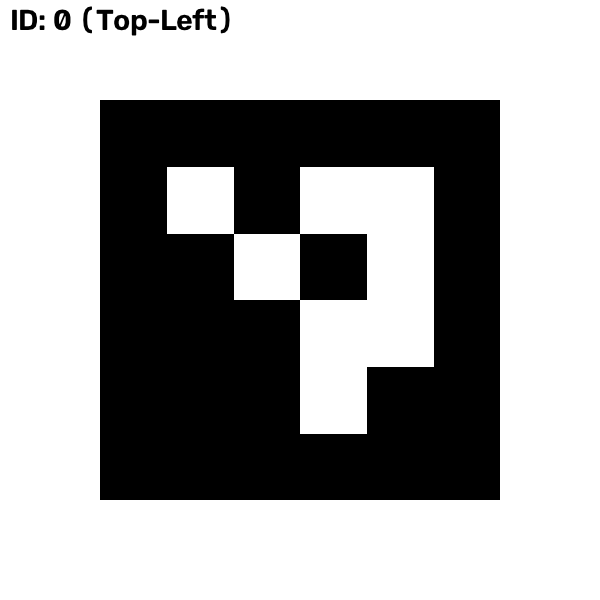
\includegraphics[width=22.5mm]{aruco/marker_0.png}};
% Top-Right (ID 1)
\node at (175.5, -12) {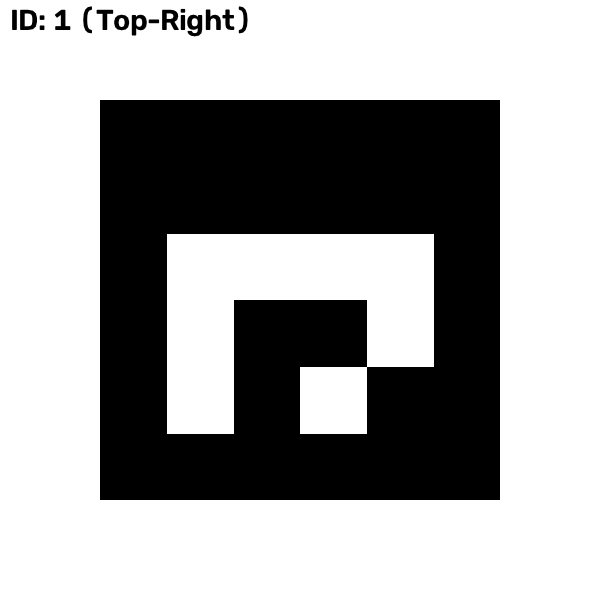
\includegraphics[width=22.5mm]{aruco/marker_1.png}};
% Bottom-Right (ID 2)
\node at (175.5, -130) {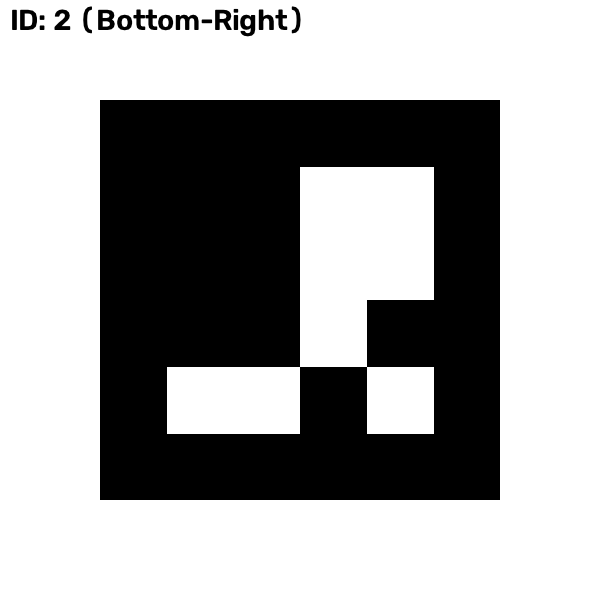
\includegraphics[width=22.5mm]{aruco/marker_2.png}};
% Bottom-Left (ID 3)
\node at (12, -130) {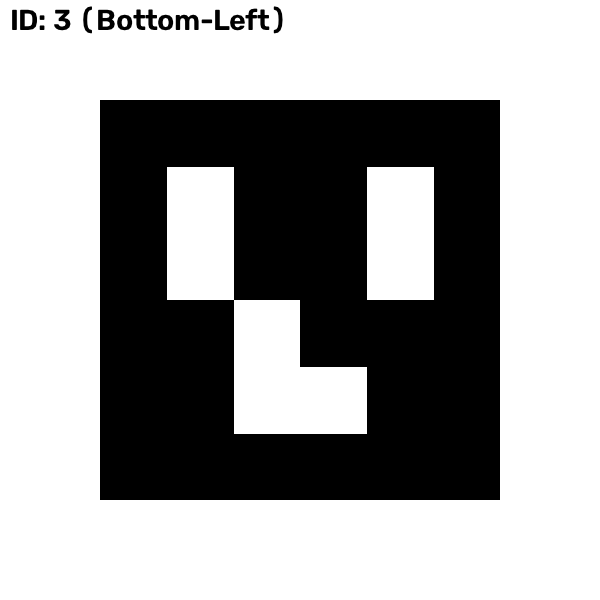
\includegraphics[width=22.5mm]{aruco/marker_3.png}};

% Middle-Left (ID 4)
\node at (12, -71) {
\includegraphics[width=22.5mm]{aruco/marker_4.png}};
% Middle-Right (ID 5)
\node at (175.5, -71) {
\includegraphics[width=22.5mm]{aruco/marker_5.png}};

% 3. Five colored circles arranged in a cross/quincunx pattern
% Center of platform: (93.75, -71)
% Spacing: ~30mm between circle centers
% Circle radius: 8mm (filled)

% Center - Blue circle
\draw[fill=blue, draw=black, thick] (93.75, -71) circle (8mm);

% Top - Black circle
\draw[fill=black, draw=black, thick] (93.75, -41) circle (8mm);

% Right - Red circle
\draw[fill=red, draw=black, thick] (123.75, -71) circle (8mm);

% Bottom - Green circle
\draw[fill=green, draw=black, thick] (93.75, -101) circle (8mm);

% Left - Yellow circle
\draw[fill=yellow, draw=black, thick] (63.75, -71) circle (8mm);

% 4. Dashed center crosshair for visual reference
\draw[gray, dashed] (93.75, -71) circle (3mm);
\draw[gray, dashed] (83.75, -71) -- (103.75, -71);
\draw[gray, dashed] (93.75, -61) -- (93.75, -81);

\end{tikzpicture}
\end{center}
\end{document}
